\documentclass{beamer}					% Document class

\usepackage[english]{babel}				% Set language
\usepackage[utf8x]{inputenc}			% Set encoding
\mode<presentation>						% Set options
{
  \usetheme{default}					% Set theme
  \usecolortheme{beaver} 				% Set colors
  \usefonttheme{default}  				% Set font theme
  \setbeamertemplate{caption}[numbered]	% Set caption to be numbered
}

% Uncomment this to have the outline at the beginning of each section highlighted.
%\AtBeginSection[]
%{
%  \begin{frame}{Outline}
%    \tableofcontents[currentsection]
%  \end{frame}
%}

\usepackage{graphicx}					% For including figures
\usepackage{booktabs}					% For table rules
\usepackage{hyperref}					% For cross-referencing

\title{Recent Education Research}	% Presentation title
\author{Joe Rowing}								% Presentation author
\institute{
\includegraphics[width=0.3\linewidth]{figures/emsnew.PNG}}					% Author affiliation
\date{\today}									% Today's date	

\begin{document}

% Title page
% This page includes the informations defined earlier including title, author/s, affiliation/s and the date
\begin{frame}
  \titlepage
\end{frame}
% Outline
% This page includes the outline (Table of content) of the presentation. All sections and subsections will appear in the outline by default.
\begin{frame}{Outline}
  \tableofcontents
\end{frame}

% The following is the most frequently used slide types in beamer
% The slide structure is as follows:
%
%\begin{frame}{<slide-title>}
%	<content>
%\end{frame}
\section{Context}
\begin{frame}{Why is it important}

``Education in the UK would benefit from a strong foundation on evidence, and the principle for basing education policy on research needs to be re-established. \textbf{\emph{The Royal Society}} believes that educational research provides the underpinning evidence to improve education, but there are sizeable gaps in knowledge and understanding.''

\note{This requires collaboration between science and mathematics education researchers, scientists, teaching professionals, policy makers and the public}
\end{frame}
\begin{frame}{Landscape of Educational Research (2021)}
  Academies commissioned research from the University of Oxford’s Department of Education to map out the landscape of educational research in the UK.
  Summary paper published this year\footnote{ \href{https://royalsociety.org/-/media/policy/projects/education-research/landscape-of-educational-research-summary-paper.pdf}{Link here}}
\end{frame}
\begin{frame}{Who pays?}
\begin{itemize}
    \item The total research funding fluctuated, with an overall increase in nominal value over the period 2010-20, and with the largest proportion of grants being of short and medium duration.
    \item Around half of the research funding for UK-led projects over the period came from the ESRC and EEF.
 \item Other major funders have included the AHRC, MRC, Nuffield Foundation and European Commission.
\end{itemize}
\end{frame}
\begin{frame}{What's being researched?}
\begin{itemize}
\item STEM Education and School-Based Intervention research are the two topics associated with the largest amount of funding.
\item The period has seen 2,440 (on average) publications and 739 (average for full years) doctoral theses per year, all covering a very wide range of topics, some of which are multi– and interdisciplinary.
\item Publications most frequently focus on education policy; learning outcomes; and teacher education; while theses most commonly address technology and education, language education, and philosophical and conceptual issues.
\item Stakeholders identified gaps in research in the following areas: curriculum design, delivery and evaluation; artificial intelligence and educational technology; initial teacher education; young people’s
voices; and longitudinal work.
\end{itemize}
\end{frame}

\section{Assessment is changing}
\begin{frame}{Assessment is changing}
    \begin{itemize}
        \item There should be a reduction in standardised tests.
     \item better, more frequent and embedded formative assessment. 
     \item development of digital portfolios and profiles.  
\end{itemize}
\begin{quote}    
Building on the work of Rethinking Assessment, the piloting of learner profiles should be extended to include a diverse range of school types and geographical areas.’ (APPG for Schools, Learning and Assessment, 2023, p. 32)
\end{quote}
\end{frame}
\begin{frame}{Rethinking assessment in schools}
    \begin{quote}
        In the last few years initiatives such as 
Rethinking Assessment (https://rethinkingassessment.com) in England,\\ New Metrics 
for Success (https://education.unimelb.edu.
au/new-metrics-for-success) in Australia,\\ and 
the Optimizing Assessment for All initiative 
of the Brookings Institution (https://www.brookings.edu) in the USA are \textbf{indicative of a global backlash against an often reductionist and deficit-based model of education}.
    \end{quote}\href{https://www.researchgate.net/publication/360806817_Rethinking_assessment_in_schools}{Get it here}
\end{frame}
\section{TeacherTapp}
\begin{frame}{Teacher Tapp}
    \begin{figure}
        \centering
        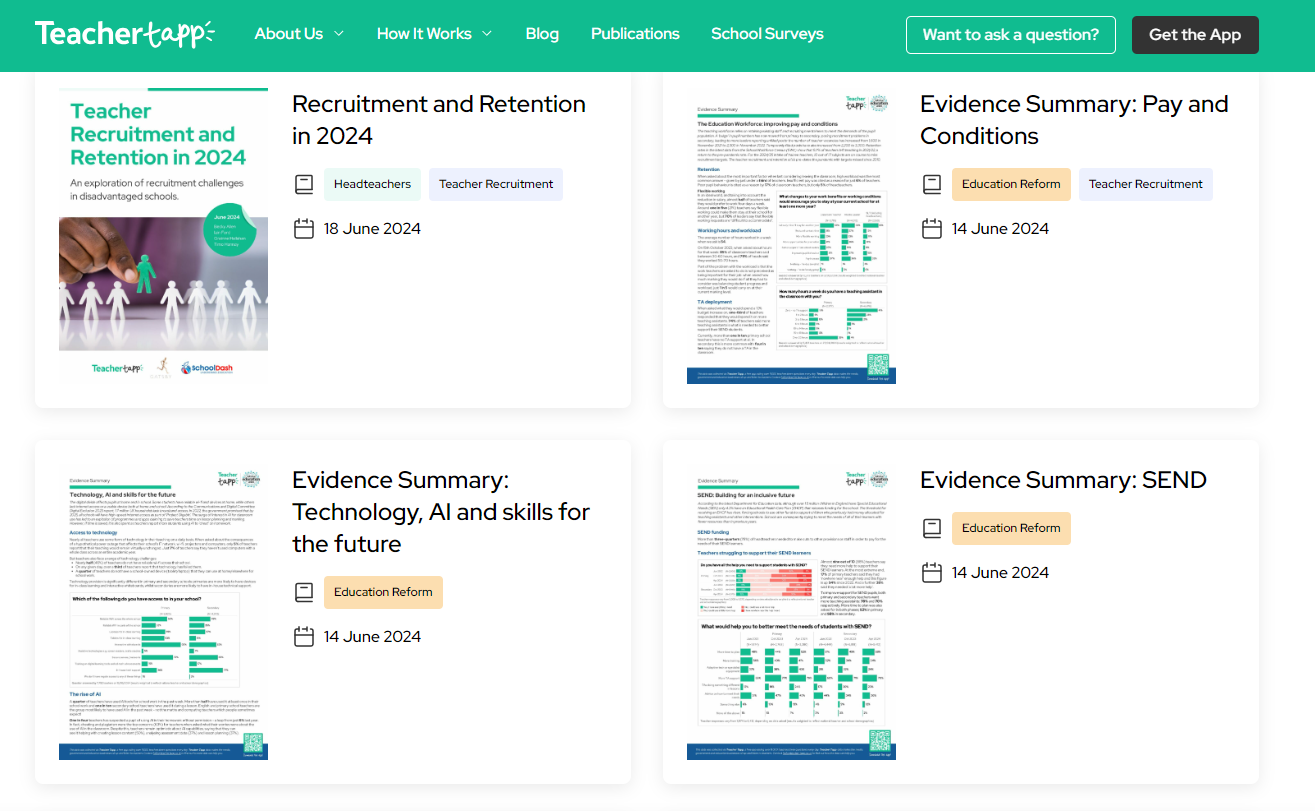
\includegraphics[width=1\linewidth]{figures/TeacherTapp.png}
        \caption{Publications based on real data(!)}
        \label{fig:enter-label}
    \end{figure}
\end{frame}

\section{AI}
\begin{frame}{AI - The Cart Before Horse}
    \begin{itemize}
    \item Pace of development outstripping ability to keep up.
     \item Chat GPT effacacy is "Mixed"
    \item Zhang et al "AI technologies for education: Recent research \& future directions" in Computers and Education: Artificial Intelligence: 
    \begin{itemize}
        \item AI is transforming educational practices - \emph{rapid} feedback, workload etc. \note{ with profound impacts across the world, including the Global South and in emergent forms of education like MOOCs, blended learning, flipped classrooms and more}
        \item Potential for SEND support fantastic.
    \end{itemize}\end{itemize}
\end{frame}
\begin{frame}{Teacher Tapp AI}
\begin{itemize}
\item A quarter of teachers have used AI tools for school work in the past week. 
\item More than half have used AI at least once in their school work 
\item One in ten secondary school teachers have used AI during a lesson. \item English and primary school teachers are the group most likely to have used AI in the past week
\item One in four teachers has suspected a pupil of using AI in their homework without permission
\end{itemize}
\end{frame}
\section{Things to try}
\begin{frame}{One thing to try}
\begin{quote}
    There is no more valuable resource than time, and there is likely no aspect of teaching that takes disproportionally more time than it has impact than giving ineffective feedback. (Hill, cited in Donarski, 2020, p. 37)
\end{quote}
\vspace{1cm}
\begin{quote}
  ‘the only important thing about feedback is what students do with it’ (Wiliam, 2016, p. 10) and that feedback should not be ‘more work for the recipient than the donor’ (Wiliam, 2011, p. 129) 
\end{quote}


\end{frame}
\begin{frame}{A Model from St Alban's High school for Girls}
    \begin{figure}
        \centering
        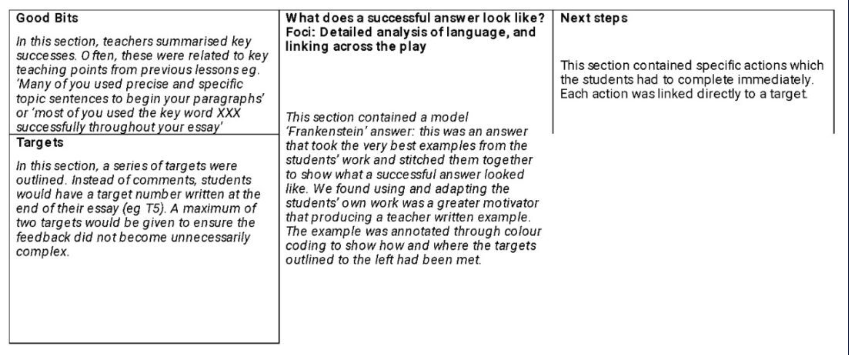
\includegraphics[width=1\linewidth]{figures/ModelFeedback.png}
        \caption{Feedback Concept}
    \end{figure}
\end{frame}
\begin{frame}{A Model from St Alban's High school for Girls}
    \begin{figure}
        \centering
        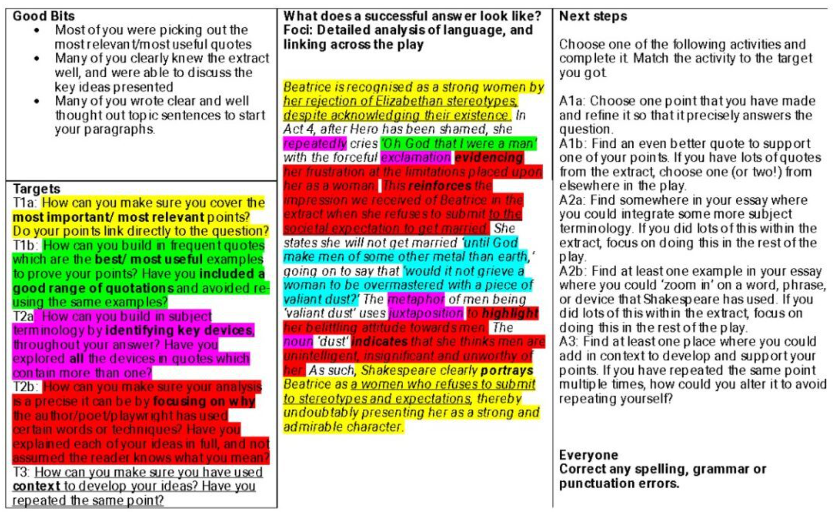
\includegraphics[width=1\linewidth]{figures/completedfeedback.png}
        \caption{Completed class feedback}
    \end{figure}
\end{frame}
\begin{frame}{Other things to do}
\begin{enumerate}
    \item Reduce biases by using rigourous Rubrics\footnote{\href{https://www.educationnext.org/wp-content/uploads/2022/01/ednext_XXI_1_quinn.pdf}{Link here}}
    \item Join \href{https://chartered.college/}{https://chartered.college/}
    \item Spaced, careful retreival practice \footnote{Agarwal PK, Nunes LD and Blunt JR (2021) Retrieval practice consistently benefits student learning: A systematic review of applied research in schools and classrooms. Educational Psychology Review 33(4):1409–1453.}
    \item Have fun with learning \footnote{Waller J (2023) The power of play: An approach to developing creativity and tolerating uncertainty. In: Imray P, Kossyvaki L and Sissons M (eds) A Different View of Curriculum and Assessment for Severe, Complex and Profound Disabilities. Abingdon and New York: Routledge, pp. 90–103.}
    \item Use Dialogic teaching
    \item Direct instruction and inquiry are complimentary
\end{enumerate}
\end{frame}
\section{The Future}
\begin{frame}{General priorities for the future of educational research}
The research in the pipeline, as suggested by reviews of ``next steps'' suggest the following themes: 
\begin{itemize}
\item AI
\item adopting a principled view on what matters in educational research; 
\item learning from past experience and models; 
\item balancing priorities and approaches; 
\item cultivating (inter/multi)disciplinarity; 
\item improving dissemination and impact and raising the profile of educational research;
\item developing and sustaining ‘capacity’ for engagement with and in 
research
\end{itemize}
\end{frame}
\end{document}
